\documentclass[aspectratio=43]{beamer}
%\usepackage[english]{babel}

%Cargar paquetes
\usepackage[utf8]{inputenc}%Permite usar acentos
\usepackage[spanish]{babel}%Configura el idioma por defecto a español
\usepackage{amsmath}%Introduce términos matemáticos
\usepackage{graphicx}%Permite introducir figuras
\usepackage[options]{natbib}%Bibliografía con estilos %No funcionan estilos en Beamer
\newcommand{\grad}{\hspace{-2mm}$\phantom{a}^{\circ}$}

\usepackage{amsthm}
\usepackage{mathtools}
\usepackage{physics}
\usepackage{calligra}
\usepackage{csquotes}
\usepackage{tensor}
\usepackage[thicklines]{cancel}
\usepackage{tcolorbox}
\usepackage{pstricks}
\usepackage[backend=biber, bibstyle=nature, sorting=nty, citestyle=numeric-comp]{biblatex} %Custom bibliography
    \addbibresource{bib.bib} %Load references


\DeclareMathAlphabet{\mathcalligra}{T1}{calligra}{m}{n}
\DeclareFontShape{T1}{calligra}{m}{n}{<->s*[2.2]callig15}{}
\newcommand{\scriptr}{\mathcalligra{r}\,}
\newcommand{\boldscriptr}{\pmb{\mathcalligra{r}}\,}
\def\rc{\scriptr}
\def\brc{\boldscriptr}
\def\hrc{\hat\brc}
\newcommand{\ie}{\emph{i.e.}} %id est
\newcommand{\eg}{\emph{e.g.}} %exempli gratia
\newcommand{\rtd}[1]{\ensuremath{\left\lfloor #1 \right\rfloor}}
\newcommand{\dirac}[1]{\ensuremath{\delta \left( #1 \right)}}
\newcommand{\diract}[1]{\ensuremath{\delta^3 \left( #1 \right)}}
\newcommand{\e}{\ensuremath{\epsilon_0}}
\newcommand{\m}{\ensuremath{\mu_0}}
\newcommand{\V}{\ensuremath{\mathcal{V}}}
\newcommand{\prnt}[1]{\ensuremath{\left(#1\right)}} %parentheses
\newcommand{\colch}[1]{\ensuremath{\left[#1\right]}} %square brackets
\newcommand{\chave}[1]{\ensuremath{\left\{#1\right\}}}  %curly brackets

\useoutertheme{infolines}
\useinnertheme{rectangles}
\usefonttheme{professionalfonts}


\definecolor{orange}{HTML}{f28165}
\definecolor{gray}{HTML}{303030}
\definecolor{yellow}{HTML}{f0be52}
\definecolor{lightorange}{HTML}{f19e58}

\renewcommand{\CancelColor}{\color{orange}}

\makeatletter
\newcommand{\mybox}[1]{%
  \setbox0=\hbox{#1}%
  \setlength{\@tempdima}{\dimexpr\wd0+13pt}%
  \begin{tcolorbox}[colback=orange,colframe=orange,boxrule=0.5pt,arc=4pt,
      left=6pt,right=6pt,top=6pt,bottom=6pt,boxsep=0pt,width=\@tempdima]
    \textcolor{white}{#1}
  \end{tcolorbox}
}
\makeatother

\usecolortheme[named=orange]{structure}
\usecolortheme{sidebartab}
\usecolortheme{orchid}
\usecolortheme{whale}
\setbeamercolor{alerted text}{fg=yellow}
\setbeamercolor{block title alerted}{bg=alerted text.fg!90!black}
\setbeamercolor{block title example}{bg=lightorange!60!black}
\setbeamercolor{background canvas}{bg=gray}
\setbeamercolor{normal text}{bg=gray,fg=white}

\setbeamertemplate{footline}
        {
      \leavevmode%
      \hbox{%
      \begin{beamercolorbox}[wd=.333333\paperwidth,ht=2.25ex,dp=1ex,center]{author in head/foot}%
        \usebeamerfont{author in head/foot}\insertshortauthor~~(\insertshortinstitute)
      \end{beamercolorbox}%
      \begin{beamercolorbox}[wd=.333333\paperwidth,ht=2.25ex,dp=1ex,center]{title in head/foot}%
        \usebeamerfont{title in head/foot}\insertshorttitle
      \end{beamercolorbox}%
      \begin{beamercolorbox}[wd=.333333\paperwidth,ht=2.25ex,dp=1ex,center]{date in head/foot}%
        \usebeamerfont{page number in head/foot}\insertframenumber/\inserttotalframenumber%\hspace*{2em}

    %#turning the next line into a comment, erases the frame numbers
        %\insertframenumber{} / \inserttotalframenumber\hspace*{2ex} 

      \end{beamercolorbox}}%
      \vskip0pt%
    }


\setbeamertemplate{blocks}[rectangle]
\setbeamercovered{dynamic}

\setbeamertemplate{section page}
{
	\begin{centering}
		\begin{beamercolorbox}[sep=27pt,center]{part title}
			\usebeamerfont{section title}\insertsection\par
			\usebeamerfont{subsection title}\insertsubsection\par
		\end{beamercolorbox}
	\end{centering}
}

%\setbeamertemplate{subsection page}
%{
%	\begin{centering}
%		\begin{beamercolorbox}[sep=12pt,center]{part title}
%			\usebeamerfont{subsection title}\insertsubsection\par
%		\end{beamercolorbox}
%	\end{centering}
%}

\newcommand{\hlight}[1]{\colorbox{violet!50}{#1}}
\newcommand{\hlighta}[1]{\colorbox{red!50}{#1}}
\title{Introducción a la Simulación} %->->->->-> Check hyperref title <-<-<-<-<-
%\subtitle{And Some Things About It}
\author[C.J. Uribe-Martes]{Carlos Javier Uribe Martes}
\institute[CUC]{
    Ingeniería Industrial%
    \\%
    Universidad de la Costa%
} %You can change the Institution if you are from somewhere else
\date{Febrero 3, 2020}
%\logo{\includegraphics[width= 0.2\textwidth]{images/a-logo.png}}

\begin{document}
    
    \frame{\titlepage}
    
    \begin{frame}{Contenido}
        \tableofcontents
    \end{frame}
    
    \section{Simulación}

\begin{frame}{Simulación}
    \begin{itemize}
        \item \textit{Simulación} se refiere a un conjunto de métodos y aplicaciones que buscan \textit{imitar} la operación de un sistema o proceso \cite{BCN,KSS}.
    \end{itemize}
\end{frame}

\begin{frame}{Simulación}
    \begin{itemize}
        \item Implica la generación de una \textit{historia artificial} del sistema \cite{BCN}.
        \item Y también la observación de dicha historia artificial para obtener inferencias relacionadas con las características operacionales del sistema \cite{BCN}.
    \end{itemize}
\end{frame}

\begin{frame}{Ventajas de la simulación}
    Dentro de las ventajas del uso de la simulación se pueden mencionar: 
    \begin{enumerate}
        \item Se puede experimentar con una variedad de escenarios, lo cual no sería posible en el sistema real \cite{KSS}.
        \item Se puede obtener una visión de la relación entre las variables y su importancia en el desempeño del sistema  \cite{BCN}.
        \item Se pueden encontrar cuellos de botellas y determinar en qué parte del proceso ocurren demoras excesivas  \cite{BCN}.
    \end{enumerate}
\end{frame}

\begin{frame}{Desventajas de la simulación}
    Algunas de las desventajas del uso de la simulación son \cite{BCN}: 
    \begin{enumerate}
        \item La construcción de modelos es un arte que requiere entrenamiento y que se aprende con la experiencia.
        \item Los resultados de los modelos de experimentación pueden ser difíciles de interpretar.
        \item Modelar y analizar un problema con simulación puede ser costoso y laborioso.
    \end{enumerate}
\end{frame}
    
    \section{Sistemas}

\begin{frame}{Sistemas}
    \begin{itemize}
        \item Un \textit{sistema} es un conjunto de elementos interdependientes que interactúan hacia el logro de un objetivo en común \cite{LK}.
        \item Durante el modelado, es necesario determinar los límites entre el sistema y su entorno. Esta decisión puede depender de los objetivos del estudio \cite{LK}.
        
    \end{itemize}
\end{frame}

\subsection{Componentes de un sistema}

\begin{frame}{Entidades}
    \begin{itemize}
        \item Una \textit{entidad} es un objeto de interés dentro del sistema.
        \item La mayoría de entidades representan objetos reales dentro del sistema. Sin embargo, en ocasiones se utilizan entidades \textit{dummies} o falsas para representar algunas situaciones dentro del sistema \cite{KSS}.
    \end{itemize}
\end{frame}

\begin{frame}{Atributos}
    \begin{itemize}
        \item Un \textit{atributo} es una propiedad de una entidad.
        \item Los atributos son características comunes para todas las entidades, pero cada entidad puede tener un valor diferente para cada característica.
    \end{itemize}
\end{frame}

\begin{frame}{Variables de estado}
    \begin{itemize}
        \item Una \textit{variable} representa un valor o característica de todo el sistema.

        \item Pueden ser escalares, vectores o matrices, suelen representar valores que cambian a lo largo de la simulación.
        
        \item Son accesibles por cualquier entidad, pertenecen al sistema y tienen un valor único en cada momento (ej: Reloj de la simulación).
    \end{itemize}
\end{frame}

\begin{frame}{Estado del sistema}
    \begin{itemize}
        \item El \textit{estado del sistema} se define como el conjunto mínimo de variables necesarias para caracterizar o describir todos aquellos aspectos de interés del sistema en un instante dado.
        
    \end{itemize}
\end{frame}

\begin{frame}{Recursos}
    \begin{itemize}
        \item Un \textit{recurso} se refiere a un servidor (operario, máquina, ubicación, etc.) capaz de ofrecer algún servicio a las entidades.
        \item Se asocia a restricciones del sistema.
        \item Las entidades compiten por el uso de los recursos. 
    \end{itemize}
\end{frame}

\begin{frame}{Actividades}
    \begin{itemize}
        \item Una \textit{actividad} representa un lapso de una duración especificada.
        \item Se asocia a menudo operaciones que demandan tiempo de uno o más recursos.
    \end{itemize}
    %------------------------
    %Incluir Listas y el Reloj
\end{frame}



\begin{frame}{Eventos}
    \begin{itemize}
        \item Un \textit{evento} se define como una ocurrencia instantánea que puede cambiar el estado del sistema.
        
        \item Durante la simulación se lleva un registro de los eventos que se espera que ocurran en el futuro; esta información se almacena en un \textit{calendario de eventos}.%\pause

    \end{itemize}
\end{frame}

\begin{frame}{Ejemplos}
\small{
\begin{table}[]
\begin{tabular}{|l|l|l|l|}
\hline
\textbf{Sistema}                                                       & Bancario                                                                                                & Producción                                                                                & Inventario                                                                     \\ \hline
\textbf{Entidad}                                                       & Cliente                                                                                                 & \begin{tabular}[c]{@{}l@{}}Órdenes de\\ producción\end{tabular}                           & Productos                                                                      \\ \hline
\textbf{Atributo}                                                      & \begin{tabular}[c]{@{}l@{}}Edad\\ Saldo en cuenta\end{tabular}                                          & \begin{tabular}[c]{@{}l@{}}Tamaño de orden\\ Prioridad del cliente\end{tabular}           & \begin{tabular}[c]{@{}l@{}}Volumen\\ Ubicación\end{tabular}                    \\ \hline
\textbf{Actividad}                                                     & Depósito                                                                                                & \begin{tabular}[c]{@{}l@{}}Soldadura\\ Maquinado\end{tabular}                             & \begin{tabular}[c]{@{}l@{}}Inspección\\ Picking\end{tabular}                   \\ \hline
\textbf{Evento}                                                        & \begin{tabular}[c]{@{}l@{}}Llegada\\ Salida\end{tabular}                                                & \begin{tabular}[c]{@{}l@{}}Falla de una \\ máquina\end{tabular}                           & \begin{tabular}[c]{@{}l@{}}Llegada de un\\ pedido\end{tabular}                 \\ \hline
\textbf{\begin{tabular}[c]{@{}l@{}}Variables\\ de estado\end{tabular}} & \begin{tabular}[c]{@{}l@{}}Número de \\ cajeros ocupados\\ Número de \\ clientes esperando\end{tabular} & \begin{tabular}[c]{@{}l@{}}Estado de \\ las máquinas\\ Producto en\\ proceso\end{tabular} & \begin{tabular}[c]{@{}l@{}}Nivel de inventario\\ Demanda atrasada\end{tabular} \\ \hline
\end{tabular}
\end{table}
}
\end{frame}

\subsection{Tipos de sistemas}

\begin{frame}{Tipos de sistemas}
\begin{columns}
\begin{column}{0.5\textwidth}
    Un sistema discreto es aquel en el cual las variables de estado cambian solo en puntos discretos en el tiempo.
\begin{figure}
    \centering
    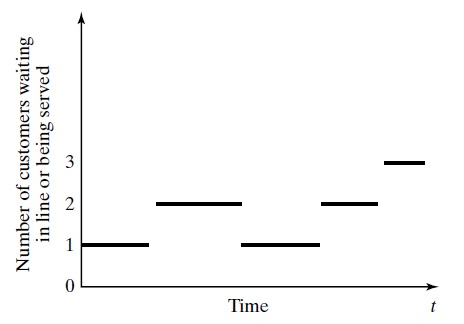
\includegraphics[width=4.5cm]{images/discreto.jpg}
    \caption{Sistema discreto}
    \label{fig:sistdiscreto}
\end{figure}
\end{column}
\begin{column}{0.5\textwidth} 
    Un sistema continuo es aquel en el cual las variables de estado cambian continuamente a lo largo del tiempo.
\begin{figure}
    \centering
    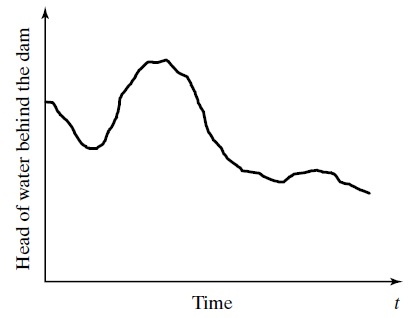
\includegraphics[width=4.5cm]{images/continuo.jpg}
    \caption{Sistema continuo}
    \label{fig:sistcontinuo}
\end{figure}
\end{column}
\end{columns}
\end{frame}




    
    \section{Modelos}

\begin{frame}{Estudio de sistemas complejos}
    La simulación es un método de estudiar un sistema complejo. Pero no es el único.
    \begin{figure}
        \centering
        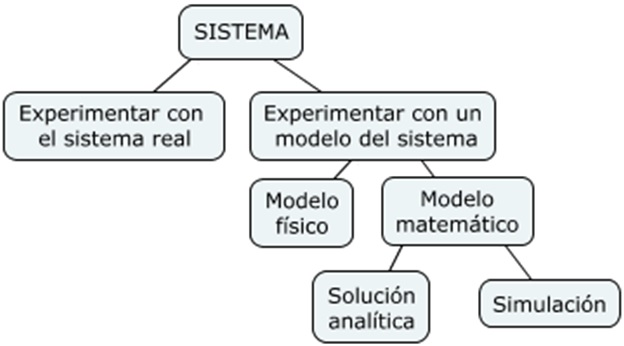
\includegraphics[width=7.5cm]{images/Sistema.jpg}
        \caption{Aproximaciones al estudio de un sistema}
        \label{fig:tipos_sol}
        %-------
        %Adapatado de LK
    \end{figure}
\end{frame}

\begin{frame}{Modelos}
    Un \textit{modelo} es definido como una representación de un sistema con el propósito de estudiarlo \cite{LK}.
\end{frame}

\begin{frame}{Tipos de Modelos}
    Los modelos pueden clasificarse de acuerdo con diferentes criterios:
    \begin{itemize}
        \item Matemáticos vs físicos.
        \item Estáticos vs dinámicos.
        \item Determinísticos vs estocásticos.
        \item Discretos vs continuos.
    \end{itemize}
\end{frame}
    
    \section*{Referencias} %You can remove this if you do not want to use it
        \begin{frame}{Referencias}
            \printbibliography
        \end{frame}
     
    \section{}   
        \begin{frame}{}
            \begin{figure}
                \centering
                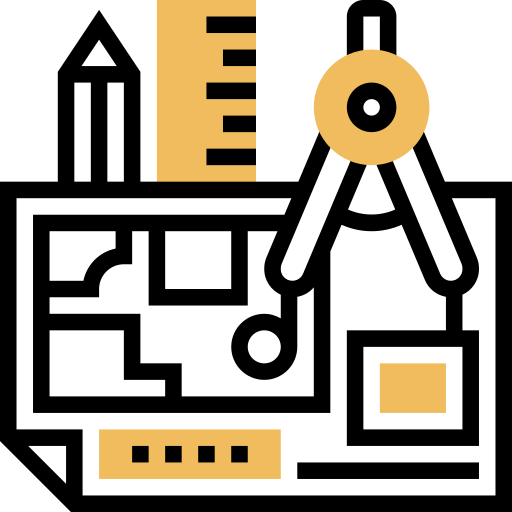
\includegraphics[width=6cm]{images/model.png}
                %\caption{Caption}
                %\label{fig:my_label}
            \end{figure}
        \end{frame}

\end{document}
